\problemname{Trevlig väg}
När jag går hemåt går jag inte alltid den kortaste vägen, utan en väg som a) hela tiden tar mig närmare hem, och b) är "trevligast", i den meningen att medelvärdet av de passerade vägavsnittens "trevlighetsfaktor" är så hög som möjligt. Skriv ett program som beräknar det maximala sådana medelvärdet.

Kartan över min stad kan beskrivas med hjälp av $n$ platser numrerade från $1$ till $n$. Plats $1$ är min startplats och plats $n$ är mitt hem, och platserna har sorterats efter avstånd så att en plats med högre nummer alltid ligger närmare hemmet än en med lägre nummer.

Vidare finns $m$ olika "vägavsnitt" som var och en leder från en plats $u_i$ till en annan plats $v_i$ och har en trevlighetsfaktor $w_i$, som kan bero på att där finns några ovanliga träd, någon gullig katt i ett fönster eller något annat trevligt. Eftersom jag alltid vill gå i riktning hemåt, så har vi i beskrivningen endast tagit med vägavsnitt där $u_i<v_i$.

Den som är lite matematiskt intresserad (ifall det nu skulle finnas någon sådan i detta sällskap) skulle kunna kalla detta för en riktad och viktad acyklisk graf.

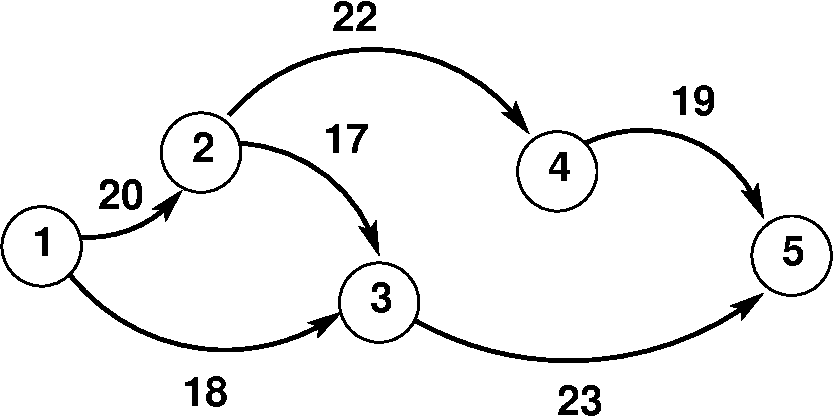
\includegraphics[width=7cm]{trevlig.pdf}\\
{\em Kartan i det andra exemplet. Den trevligaste vägen är $1\rightarrow 3\rightarrow 5$.}

%Vi har givet en riktad graf med N noder och M viktade kanter. Alla kanter pekar från lägre index till större.
%Vilket är det högsta medelvärde som kan uppnås av en väg från nod 1 till nod N?

\section*{Indata}
Den första raden innehåller de två heltalen $n$ och $m$ ($2 \leq n \leq 10^5$ , $1 \leq m \leq 2\cdot 10^5$).
Var och en av de följande $m$ raderna beskriver ett vägavsnitt och innehåller tre heltal $u_i$, $v_i$ och $w_i$ ($1 \leq u_i < v_i \leq n$, $1 \le w_i \le 2\cdot 10^6$),
vilket betyder att vägavsnittet går från plats $u_i$ till plats $v_i$ och har trevlighetsfaktor $w_i$.

Det kommer aldrig finnas mer än ett vägavsnitt som förbinder samma platser, och det garanteras
att det går att ta sig från plats $1$ till plats $n$.

\section*{Utdata}
Skriv ut ett tal: det högsta uppnåbara medelvärdet av trevlighetsfaktorer på en väg från plats 1 till plats $n$.
Svaret anses korrekt om det har ett relativt eller absolut fel av högst $10^{-6}$.

\section*{Poängsättning}
Din lösning kommer att testas på en mängd testfallsgrupper. För att få poäng för en grupp så måste du klara alla testfall i gruppen.

\noindent
\begin{tabular}{| l | l | l |}
\hline
Grupp & Poängvärde & Gränser \\ \hline
1     & 21         &  $2 \le n \le 10$ , $1 \le m \le 20$ \\ \hline
2     & 41         &  $2 \le n \le 1000$ , $1 \le m \le 2000$ \\ \hline
3     & 38         & Inga ytterligare begränsningar \\ \hline
\end{tabular}
